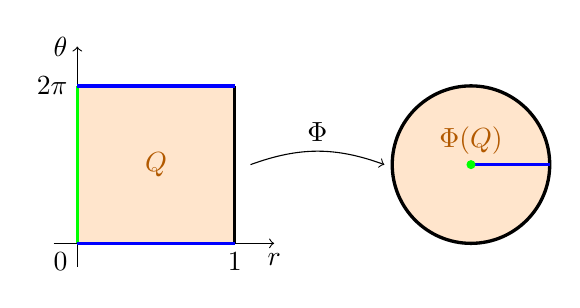
\begin{tikzpicture}
\fill[orange!20!white] (0,0) rectangle (2,2);

\draw[->] (0,-0.3) -- (0,2.5);
\node[left] at (0,2.5) {$\theta$};
\node[left] at (0,2) {$2\pi$};
\draw[->] (-0.3,0) -- (2.5,0);
\node[below] at (2.5,0) {$r$};
\node[below] at (2,0) {$1$};
\node[below left] at (0,0) {$0$};

\draw[very thick] (2,0) -- (2,2);
\draw[very thick,green] (0,0) -- (0,2);
\draw[very thick,blue] (0,2) -- (2,2);
\draw[very thick,blue] (0,0) -- (2,0);

\node[orange!70!black] at (1,1) {$Q$};

\draw[->] (2.2,1) to[out=20,in=160] node[midway,above,sloped] {$\Phi$} (3.9,1);

\draw[very thick,fill=orange!20!white] (5,1) circle (1);
\draw[very thick,blue] (5,1) -- (6,1);
\node[inner sep=1pt,circle,green,draw,fill=green] at (5,1) {};

\node[orange!70!black, above] at (5,1) {$\Phi(Q)$};

\end{tikzpicture}